%%%%% Paramétrage du cours %%%%
%\def\xxactivite{Cours}
%\def\xxauteur{\textsl{Xavier Pessoles}}
%
%\fichetrue
%\proftrue
%\tdfalse
%\setchapterimage{Header_Peugeot.jpg}
%\setchapterpreamble[u]{\margintoc}
%%\setcounter{chapter}{1}
%
%\chapter{Résolution d'un problème de statique}

\marginnote[3cm]{
%\UPSTIcompetence[2]{C1-05}
%\UPSTIcompetence[2]{C2-07}
%\UPSTIcompetence[2]{C2-03}
\xpComp{STAT}{01}
\xpComp{STAT}{03}
}


\setcounter{section}{0}
\section{Ce qu'il faut connaître et savoir faire... pour pouvoir commencer}
\begin{enumerate}
\item \textbf{Les torseurs des actions mécaniques dans les liaisons.}
\item \textbf{Faire un bilan des actions mécaniques extérieures et écrire le torseur associé.}
\item Les torseurs des actions mécaniques dans les liaisons.
\item \textbf{Faire un graphe d'analyse (ou de structure : liaisons et actions mécaniques extérieures).}
\item Les torseurs des actions mécaniques dans les liaisons.
\item \textbf{Faire des produits vectoriels le plus vite possible.}
\item Les torseurs des actions mécaniques dans les liaisons.
\item \textbf{Simplifier les torseurs des actions mécaniques dans les liaisons dans le cas d'un problème plan}.
\end{enumerate}



\section{Les types de problèmes}

Le principe fondamental de la statique a pour objectif de calculer des actions mécaniques dans deux cas :
\begin{enumerate}
\item \textbf{connaître toutes les actions mécaniques dans toutes les liaisons;}
\item \textbf{connaître la loi entrée-sortie en effort}, c'est à dire :
\begin{itemize}
\item quel couple moteur faut-il pour déplacer un objet ?
\item quel effort doit fournir le vérin pour soulever cette masse ?
\item ...
\end{itemize}
\end{enumerate}

Dans le cas 1, il faut isoler chacune des pièces et réaliser le PFS. 

Dans le cas 2, on peut essayer de minimiser le nombre d'équations à écrire. C'est cette stratégie que nous allons présenté.


\section{Stratégie d'isolement}

\subsection{Graphe d'analyse, ou de structure}
\marginnote{\xpComp{STAT}{01}\xpComp{STAT}{03}}
On rencontre principalement deux types de structures : des chaînes fermées, ou des chaînes ouvertes.

\begin{figure*}[!ht]
\begin{minipage}[c]{.4\linewidth}
\begin{center}
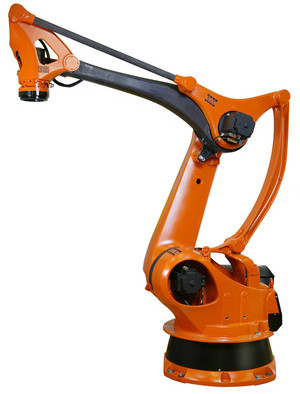
\includegraphics[width=\linewidth]{fig_01}
\end{center}
\end{minipage}
\hfill
\begin{minipage}[c]{.55\linewidth}
\begin{center}
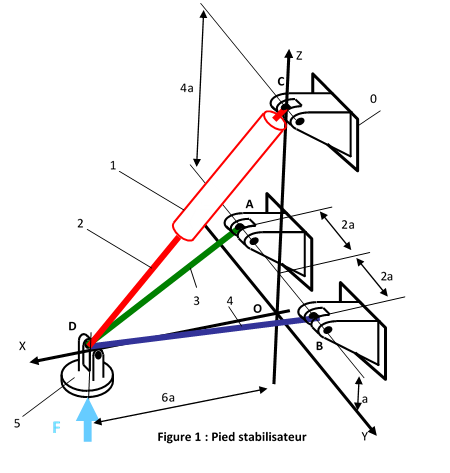
\includegraphics[width=\linewidth]{fig_02}
\end{center}
\end{minipage}
\end{figure*}

\textbf{Remarques :}
\begin{itemize}
\item Entre les pièces (ou les groupes de pièces), on matérialise les liaisons (dont vous connaissez super bien les torseurs).
\item Entre certaines pièces (ou groupes de pièces), il peut exister des actions mécaniques extérieures qui agissent << en positif >> sur une des pièces et << en négatif >> sur l'autre. \textbf{C'est par exemple le cas des moteurs et des vérins}. Il faut bien préciser que l'action mécanique agit sur les deux pièces.
\item Les actions strictement extérieures (comme la pesanteur) ne sont pas en interactions entre deux pièces.
\end{itemize}


\subsection{Isoler les solides soumis à 2 glisseurs}

On commence toujours, \large{toujours}, \Large{toujours}, \LARGE{toujours}, \huge{toujours} \normalsize par isoler les ensembles soumis à 2 glisseurs. Cela permet de conclure que, d'après le PFS (et le principe des actions réciproques qui en découle) les actions mécaniques agissant sur ce solide ont même direction, même norme et sens opposé. Ce qui supprime des inconnues.

\textbf{Mais qu'est-ce qu'un glisseur ?}

Un glisseur est un torseur dont-il existe un point tel que le moment est nul. Ainsi, le torseur statique d'une lisaison rotule est un glisseur. Le torseur statique d'une liaison pivot n'est pas un glisseur. 

%Lorsque le problème est plan est une liaison pivot à son axe perpendiculaire au plan, c'est un glisseur. 

%Le torseur cinématique d'une glissière est un glisseur... alors que le torseur statique d'une liaison glissière ne l'est pas... 


\begin{remarque}
Pour démontrer qu'un torseur est un glisseur, on peut par exemple montrer que son automoment est nul. L'automoment est le produit de la résultante et du moment d'un torseur. Il est identique en tout point. C'est un invariant du torseur (comme la résultante).
\end{remarque}


Dans le cas ci-contre, si on isole 2, 3 et $h$ (qui pourrait être une action hydraulique). Ainsi, si $\left\{\mathcal{T}_{12}\right\}$ et $\left\{\mathcal{T}_{43}\right\}$ sont des glisseurs de << centres >> respectifs $A$ et $B$ et qu'on note $\vect{u}=\dfrac{\vect{AB}}{||\vect{AB}||}$. Alors on a $\left\{\mathcal{T}_{12}\right\}=-\left\{\mathcal{T}_{43}\right\}=\torseurl{F\vect{u}}{\vect{0}}{A}$. 
\begin{marginfigure}
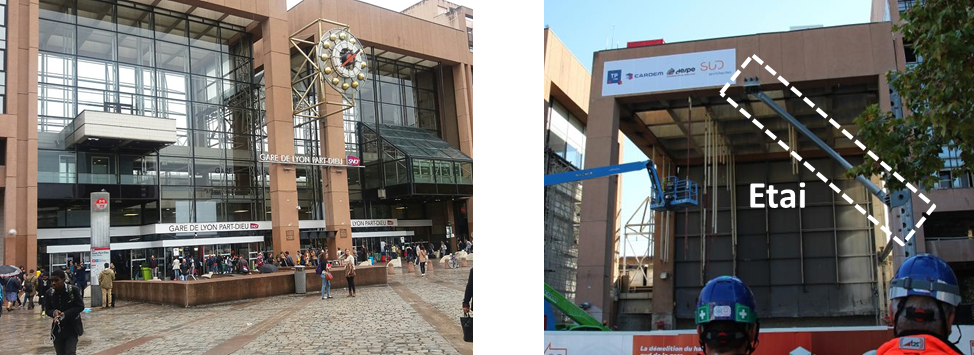
\includegraphics[width=\linewidth]{fig_03}
\end{marginfigure}


\textbf{Il faut bien comprendre que $\left\{\mathcal{T}_{12}\right\}$ et $\left\{\mathcal{T}_{43}\right\}$  pouvaient avoir chacun 2 ou 3 inconnues et que maintenant nous avons au total UNE inconnue.}


\subsection{Isoler les solides soumis à 3 glisseurs ou plus}

La stratégie est toujours la suivante :
\begin{enumerate}
\item \textbf{Isoler la pièce.}
\item \textbf{Réaliser le bilan des actions mécaniques, en écrivant les torseurs} et en laissant de la place à gauche de la feuille pour les déplacer.
\item \textbf{Citer L'équation du PFS qu'on va utiliser.} Cela peut être le théorème de la résultante statique (TRS) suivant l'axe $\vect{u}$ ou le théorème du moment statique (TMS) au point $A$ en projection sur $\vect{u}$.
\item \textbf{Effectuer la résolution.} (Déplacer les torseurs, appliquer le PFS.)
\item \textbf{Réitérer avec un autre isolement.}
\end{enumerate}

\subsection{Oui, mais quel est le problème ?}

Le problème est de choisir \textbf{\large{L'}}\normalsize équation. Je dirai qu'il faut écrire le théorème qui correspond à la mobilité de la pièce isolée, mais cela a-t-il vraiment un sens ? Prenons des exemples...

\begin{marginfigure}
\begin{center}
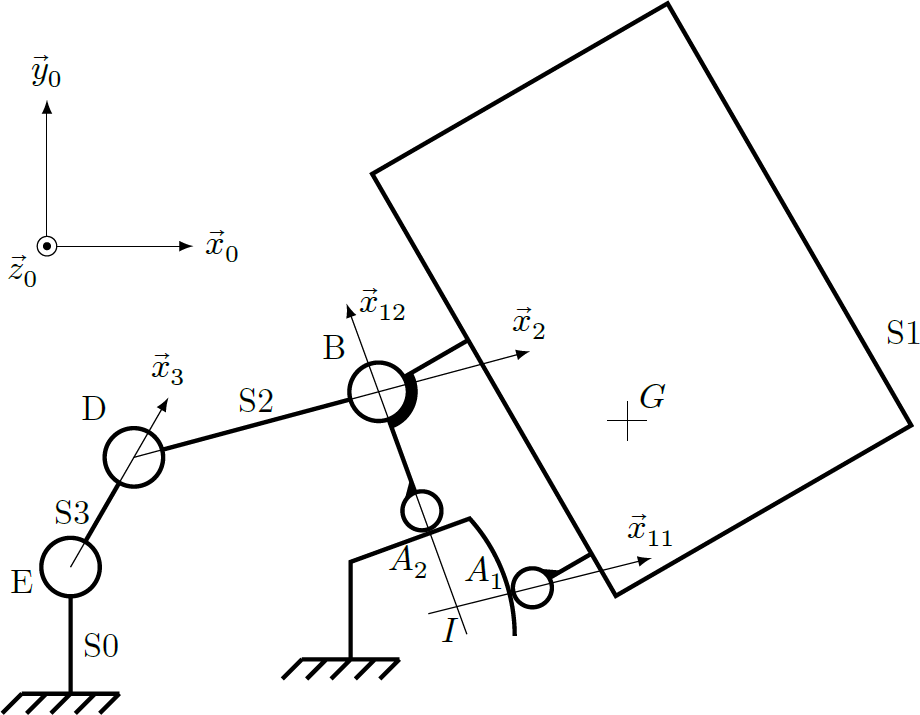
\includegraphics[width=\linewidth]{fig_04}
\end{center}
\end{marginfigure}

Si on a isolé 4 et que  $\left\{\mathcal{T}_{14}\right\}$ est une liaison pivot d'axe $\axe{A}{z}$, on réalisera un théorème du moment statique en $A$ en projection suivant $\vect{z}$.

Si on a isolé 4 et que  $\left\{\mathcal{T}_{14}\right\}$ est une liaison glissière de direction $\vect{u}$, on réalisera un théorème de la résultante statique en projection suivant $\vect{u}$.

... \textbf{Est-ce que c'est plus clair ?}... J'espère...





\begin{marginfigure}[4cm]
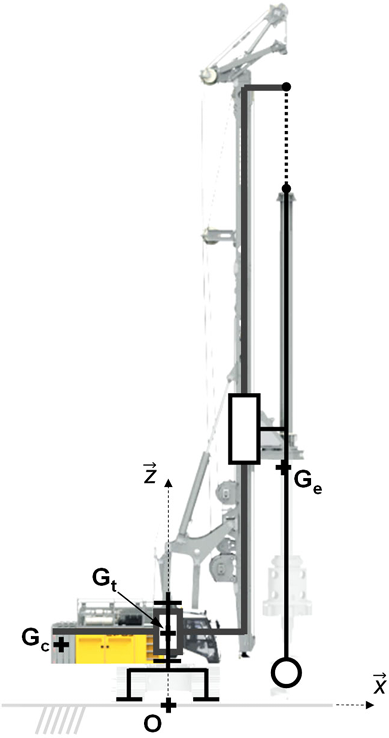
\includegraphics[width=\linewidth]{fig_05}
\end{marginfigure}

Si on cherche une relation entre l'effort extérieur et $C_{m2}$, que la liaison entre 2 et 3 est une liaison pivot d'axe 
$\axe{B}{x}$, on isolera \textbf{\{3 et 4\}} et on réalisera un théorème du moment statique en $B$ en projection suivant $\vect{x}$.

... \textbf{Toujours pas clair ?}... Si ?



\subsection{Il y a plus qu'à ...}

Petite remarque pour finir : le produit mixte. Lorsqu'on applique un TMS suivant une direction, le produit mixte peut être un bon outil :
$\vectm{B}{1}{2}\cdot \vect{z} = \left( \vectm{A}{1}{2} + \vect{BA}\wedge \vectf{1}{2}\right)\cdot \vect{z}$
$=  \vectm{A}{1}{2}\cdot \vect{z} + \left(\vect{BA}\wedge \vectf{1}{2}\right)\cdot \vect{z}$...
et $\left(\vect{u} \wedge \vect{v}\right) \cdot \vect{z}= \left(\vect{v} \wedge \vect{z}\right) \cdot \vect{u}= \left(\vect{z} \wedge \vect{u}\right) \cdot \vect{v}$.